\section{Durchführung}
\label{sec:Durchführung}
\begin{figure}[H]
  \centering
  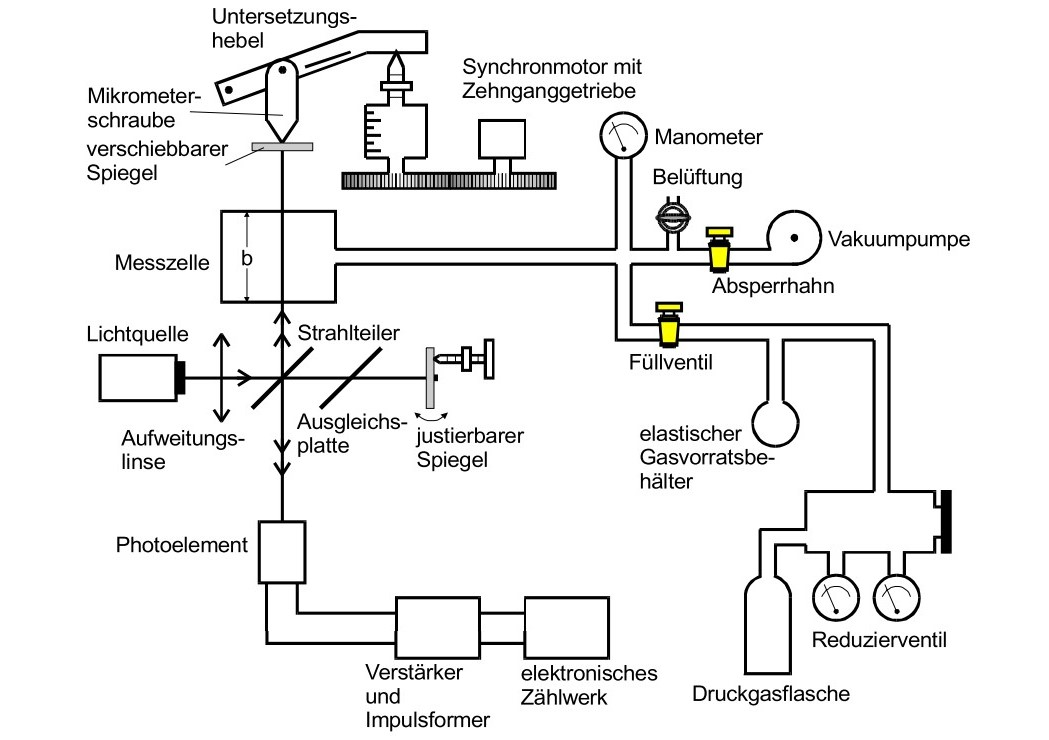
\includegraphics[scale=0.8]{aparatur.jpg}
  \caption{Darstellung der gesamten Messapparatur \cite{Anleitung}.}
  \label{fig:aparatur}
\end{figure}
Der Aufbau des Versuchs ist Abbildung \ref{fig:aparatur} zu entnehmen. Zunächst müssen die Spiegel mithilfe des Lasers so justiert werden,
dass die beiden hellsten aus der Interferometer austretenden Strahlen am Detektor zur Deckung gebracht werden. Hierfür
wird eine Mattscheibe verwendet. Das Photoelement, welches zur Vereinfachung der Zählung genutzt wird, 
wird dann auf die entsprechende Höhe eingestellt, sodass das Interferenzbild genau auf den Eintrittspalt
fällt. Für eine möglichst genaue Messung der Wellenlänge wird der zu verschiebende Spiegel mit einem feinen Synchronmotor bewegt.
Der Spiegel wird zehn mal so weit verschoben, dass mindestens 3000 Maxima zu zählen sind, da die Wellenlänge des Lasers
klein im Verhältnis zur Verschiebung des Spiegels ist und die Verschiebung wird notiert. \\
Um den Brechungsindex von Luft zu bestimmen, wird der Innendruck $p$ der Messzelle der Dicke $b = 50\,\si{\milli\meter}$ mit einer
Vakuumpumpe auf $p' = 0,4\,\si{\bar}$ verringert. Beim Wiedereinlassen der Luft werden erneut Interferenzmaxima gezählt, die notiert werden.